\documentclass{article}

% Page/layout
\usepackage[a4paper,margin=1in]{geometry}

% Math and symbols
\usepackage{amsmath,amssymb,mathtools}

% Figures, tables, lists, columns
\usepackage{graphicx,booktabs,multicol,enumitem}

% Units and code listings helpers used by gvv
\usepackage{siunitx}
\usepackage{xcolor,listings,xparse}

% Your styles (define \brak, \sbrak, etc.)
\usepackage{gvv}
\usepackage{gvv-book}

% If you want T1 encoding with txfonts (from gvv-book), this is fine:
\usepackage[T1]{fontenc}

\usepackage{noto}

\title{GATE 2016 Mining Engineering (MN)}
\author{AI25BTECH11039 — Harichandana Varanasi\textsuperscript{*}}
\date{August 10, 2025} % or \today


% Bracket helpers
\usepackage{mathtools} % loads amsmath


\begin{document}

\begin{center}
    \textbf{\Large GATE 2016}
\end{center}

\section*{General Aptitude - GA Set-2}

\subsection*{Q. 1 -- Q. 5 carry one mark each}

\begin{enumerate}[label=\textbf{Q.\arabic*}, leftmargin=*]
    \item The volume of a sphere of diameter 1 unit is \underline{\hspace{1cm}} than the volume of a cube of side 1 unit.
    \begin{enumerate}[label=(\Alph*)]
        \item least
        \item less
        \item lesser
        \item low
    \end{enumerate}

    \item The unruly crowd demanded that the accused be \underline{\hspace{1cm}} without trial.
    \begin{enumerate}[label=(\Alph*)]
        \item hanged
        \item hanging
        \item hankering
        \item hung
    \end{enumerate}

    \item Choose the statement(s) where the underlined word is used correctly:
    \begin{enumerate}[label=(i)]
        \item A \underline{prone} is a dried plum.
        \item He was lying \underline{prone} on the floor.
        \item People who eat a lot of fat are \underline{prone} to heart disease.
    \end{enumerate}
    \begin{enumerate}[label=(\Alph*)]
        \item (i) and (iii) only
        \item (iii) only
        \item (i) and (ii) only
        \item (ii) and (iii) only
    \end{enumerate}

    \item Fact: If it rains, then the field is wet.\\
    Read the following statements:
    \begin{enumerate}[label=(i)]
        \item It rains
        \item The field is not wet
        \item The field is wet
        \item It did not rain
    \end{enumerate}
    Which one of the options given below is NOT logically possible, based on the given fact?
    \begin{enumerate}[label=(\Alph*)]
        \item If (iii), then (iv).
        \item If (i), then (iii).
        \item If (i), then (ii).
        \item If (ii), then (iv).
    \end{enumerate}

    \item A window is made up of a square portion and an equilateral triangle portion above it. The base of the triangular portion coincides with the upper side of the square. If the perimeter of the window is 6 m, the area of the window in \si{\metre\squared} is \underline{\hspace{1cm}}.
    \begin{enumerate}[label=(\Alph*)]
        \item 1.43
        \item 2.06
        \item 2.68
        \item 2.88
    \end{enumerate}
\end{enumerate}

\subsection*{Q. 6 -- Q. 10 carry two marks each}

\begin{enumerate}[label=\textbf{Q.\arabic*}, leftmargin=*, resume]
    \item Students taking an exam are divided into two groups, P and Q such that each group has the same number of students. The performance of each of the students in a test was evaluated out of 200 marks. It was observed that the mean of group P was 105, while that of group Q was 85. The standard deviation of group P was 25, while that of group Q was 5. Assuming that the marks were distributed on a normal distribution, which of the following statements will have the highest probability of being TRUE?
    \begin{enumerate}[label=(\Alph*)]
        \item No student in group Q scored less marks than any student in group P.
        \item No student in group P scored less marks than any student in group Q.
        \item Most students of group Q scored marks in a narrower range than students in group P.
        \item The median of the marks of group P is 100.
    \end{enumerate}

    \item A smart city integrates all modes of transport, uses clean energy and promotes sustainable use of resources. It also uses technology to ensure safety and security of the city, something which critics argue, will lead to a surveillance state.\\
    Which of the following can be logically inferred from the above paragraph?
    \begin{enumerate}[label=(i)]
        \item All smart cities encourage the formation of surveillance states.
        \item Surveillance is an integral part of a smart city.
        \item Sustainability and surveillance go hand in hand in a smart city.
        \item There is a perception that smart cities promote surveillance.
    \end{enumerate}
    \begin{enumerate}[label=(\Alph*)]
        \item (i) and (iv) only
        \item (ii) and (iii) only
        \item (iv) only
        \item (i) only
    \end{enumerate}

    \item Find the missing sequence in the letter series.\\
    B, FH, LNP, \underline{\hspace{1cm}}.
    \begin{enumerate}[label=(\Alph*)]
        \item SUWY
        \item TUVW
        \item TVXZ
        \item TWXZ
    \end{enumerate}

    \item The binary operation $\square$ is defined as $a \square b = ab + (a + b)$, where $a$ and $b$ are any two real numbers. The value of the identity element of this operation, defined as the number $x$ such that $a \square x = a$, for any $a$, is \underline{\hspace{1cm}}.
    \begin{enumerate}[label=(\Alph*)]
        \item 0
        \item 1
        \item 2
        \item 10
    \end{enumerate}

    \item Which of the following curves represents the function $y = \ln(|\mathrm{e}^{x} + \mathrm{e}^{|x|}|)$ for $|x| < 2\pi$? Here, $x$ represents the abscissa and $y$ represents the ordinate.
        \begin{center}
      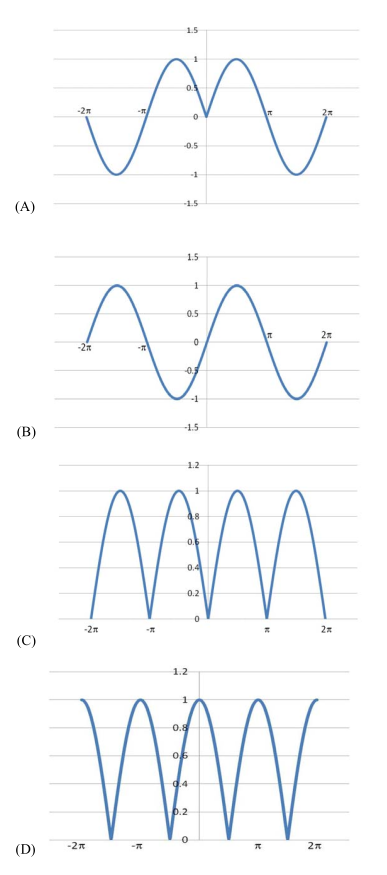
\includegraphics[width=0.8\linewidth]{images/1.png}
    \end{center}
\end{enumerate}

\section*{Mining Engineering (MN)}

\subsection*{Q. 1 -- Q. 25 carry one mark each}

\begin{enumerate}[label=\textbf{Q.\arabic*}, leftmargin=*]
    \item The differential of the equation, $\frac{y^2}{x^2} + 1 = 0$, with respect to $x$ is
    \begin{enumerate}[label=(\Alph*)]
        \item $- \frac{x}{y}$
        \item $\frac{x}{y}$
        \item $- \frac{y}{x}$
        \item $\frac{y}{x}$
    \end{enumerate}

    \item If $\sbrak{A} \sbrak{B} = \sbrak{I}$ then
    \begin{enumerate}[label=(\Alph*)]
        \item $\sbrak{B} = \sbrak{A}^T$
        \item $\sbrak{A} = \sbrak{B}^T$
        \item $\sbrak{B} = \sbrak{A}^{-1}$
        \item $\sbrak{B} = \sbrak{A}$
    \end{enumerate}

    \item $x^4 + C$ is the general integral of
    \begin{enumerate}[label=(\Alph*)]
        \item $\int 3x^3 \, dx$
        \item $\int \frac{1}{4} x^3 \, dx$
        \item $\int 3x \, dx$
        \item $\int 4 x^3 \, dx$
    \end{enumerate}

    \item $\sinh(x)$ is
    \begin{enumerate}[label=(\Alph*)]
        \item $\frac{e^x - e^{-x}}{4}$
        \item $\frac{e^x - e^{-x}}{2}$
        \item $\frac{e^x + e^{-x}}{2}$
        \item $\frac{e^x + e^{-x}}{4}$
    \end{enumerate}

    \item Identify the correct statement. NONEL is used for surface connection of the blast holes in order to
    \begin{enumerate}[label=(\Alph*)]
        \item achieve better water resistance over detonating fuse
        \item have a precise delay timing
        \item provide noiseless shock front movement
        \item avoid deflagration
    \end{enumerate}

    \item Identify the pattern of surface blasting given in the figure. The values of delay time, in ms, are given against each blasthole.
    \begin{center}
        \begin{center}
      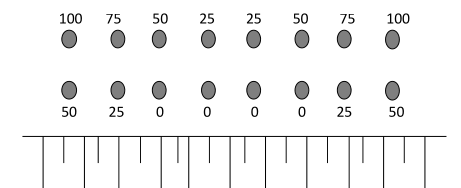
\includegraphics[width=0.8\linewidth]{images/2.png}
    \end{center}
    \end{center}
    \begin{enumerate}[label=(\Alph*)]
        \item V-cut
        \item extended V-cut
        \item row to row
        \item en echelon
    \end{enumerate}

    \item Identify the initiation sequence which is NOT possible for surface blasting.
    \begin{enumerate}[label=(\Alph*)]
        \item Detonating fuse $\to$ Nonel $\to$ Electronic detonator
        \item Electric detonator $\to$ Nonel $\to$ Detonating fuse
        \item Electric detonator $\to$ Detonating fuse $\to$ Nonel
        \item Electronic detonator $\to$ Detonating fuse $\to$ Nonel
    \end{enumerate}

    \item Parallel holes at right angles to the face with some holes uncharged are associated with the following shot hole pattern
    \begin{enumerate}[label=(\Alph*)]
        \item drag cut
        \item wedge cut
        \item pyramid cut
        \item burn cut
    \end{enumerate}

    \item Bieniawski’s Rock Mass Rating considers the parameters: RQD, spacing of joints, condition of joints, ground water condition, and
    \begin{enumerate}[label=(\Alph*)]
        \item tensile strength
        \item uniaxial compressive strength
        \item shear strength
        \item buckling strength
    \end{enumerate}

    \item A rockmass is subjected to hydrostatic pressure of 6 MPa. If each of the measured strains $\epsilon_{xx} = \epsilon_{yy} = \epsilon_{zz}$ is 2.0 mm/m, then the bulk modulus, in GPa, is \underline{\hspace{1cm}}.

    \item Identify the uniaxial compressive loading condition from the following four Mohr circles.
        \begin{center}
      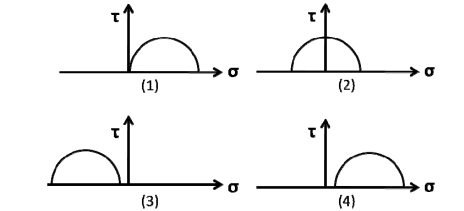
\includegraphics[width=0.8\linewidth]{images/3.png}
    \end{center}
    \begin{enumerate}[label=(\Alph*)]
        \item (1)
        \item (2)
        \item (3)
        \item (4)
    \end{enumerate}

    \item Out of the given stress-strain curves, identify the rock type that is most prone to rock burst.
    \begin{center}
      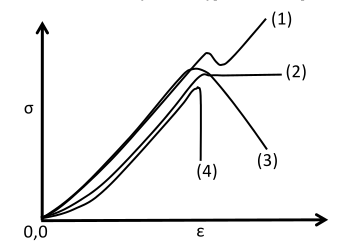
\includegraphics[width=0.8\linewidth]{images/4.png}
    \end{center}
    \begin{enumerate}[label=(\Alph*)]
        \item (1)
        \item (2)
        \item (3)
        \item (4)
    \end{enumerate}

    \item A longwall panel of width 120 m is extracted at a depth of 200 m. Critical subsidence is reached when the panel length becomes 150 m. If the seam were to be worked at a depth of 300 m, critical subsidence would be observed at a panel length, in m, of \underline{\hspace{1cm}}.

    \item The support system followed along the goaf edge in a depillaring panel is
    \begin{enumerate}[label=(\Alph*)]
        \item rope stitching
        \item cable bolting
        \item wooden/steel chock
        \item hydraulic prop
    \end{enumerate}

    \item Which one of the following ropes CANNOT be an effective cable bolt?
    \begin{enumerate}[label=(\Alph*)]
        \item locked coil wire rope
        \item Langs lay wire rope
        \item ordinary lay wire rope
        \item bird-caged wire rope
    \end{enumerate}

    \item In metalliferous mines, the sublevel interval does NOT depend on
    \begin{enumerate}[label=(\Alph*)]
        \item capacity of drilling equipment
        \item capacity of loading equipment
        \item strength of rib pillar
        \item strength of wall rock
    \end{enumerate}

    \item Jack hammer does NOT contain
    \begin{enumerate}[label=(\Alph*)]
        \item pawl and ratchet
        \item gear box
        \item rifle bar
        \item piston
    \end{enumerate}

    \item At the inlet of a mine roadway, the dry and wet bulb temperatures of air are \SI{38}{\celsius} and \SI{29}{\celsius}, respectively. At the outlet, the corresponding temperatures are \SI{32}{\celsius} and \SI{29}{\celsius}, respectively. The process of heat transfer in the airway is described as
    \begin{enumerate}[label=(\Alph*)]
        \item evaporative cooling
        \item sensible cooling
        \item sensible heating
        \item dehumidification
    \end{enumerate}

    \item Underground coal mines are in principle ventilated by exhausting system, so that
    \begin{enumerate}[label=(\Alph*)]
        \item spontaneous heating risk is reduced
        \item fumes can be quickly removed in case of an underground fire
        \item build-up of methane concentration is decreased
        \item cool and fresh intake air can enter underground
    \end{enumerate}

    \item Identify the WRONG statement. Pit bottom air lock
    \begin{enumerate}[label=(\Alph*)]
        \item prevents the short circuiting of air when the flow is reversed in coal mines
        \item has at least three doors
        \item has at least one door that has provision for latching
        \item all doors are in principle designed to open towards high pressure side of the air
    \end{enumerate}

    \item Identify the WRONG statement. The ‘temperature inversion’ of the atmosphere in surface mines aggravates the problem of
    \begin{enumerate}[label=(\Alph*)]
        \item airborne dust
        \item noise
        \item ground vibrations
        \item visibility
    \end{enumerate}

    \item In a CO self rescuer, the purpose of the calcium bromide and lithium chloride mixture is to
    \begin{enumerate}[label=(\Alph*)]
        \item dry the incoming air
        \item convert the CO catalytically to CO$_2$
        \item absorb and thereby neutralise CO
        \item cool the inhaled air from excess exothermic heat due to chemical reaction
    \end{enumerate}

    \item IRR of a project is the discount rate at which
    \begin{enumerate}[label=(\Alph*)]
        \item profit after tax is zero
        \item written down value of the project is zero
        \item revenue from the project is zero
        \item NPV is zero
    \end{enumerate}

    \item For the critical path network shown, the slack for the activity ‘b’, in months, is
        \begin{center}
      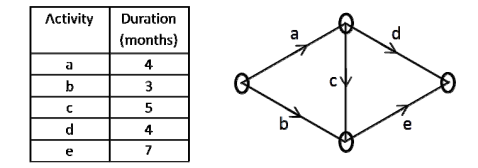
\includegraphics[width=0.8\linewidth]{images/5.png}
    \end{center}
    \begin{enumerate}[label=(\Alph*)]
        \item 4
        \item 6
        \item 9
        \item 13
    \end{enumerate}

    \item The three axes comprising the numerical codification of resources, as per the UNFC, are
    \begin{enumerate}[label=(\Alph*)]
        \item Economic Viability, Geological Assessment, Geotechnical Assessment
        \item Geological Assessment, Environmental Assessment, Feasibility Assessment
        \item Feasibility Assessment, Geological Assessment, Mining Assessment
        \item Economic Viability, Geological Assessment, Feasibility Assessment
    \end{enumerate}
\end{enumerate}

\subsection*{Q. 26 -- Q. 55 carry two marks each}

\begin{enumerate}[label=\textbf{Q.\arabic*}, leftmargin=*, resume]
    \item Equations of two planes are $z = 4$ and $z = 3x + 4$. The included angle between the two planes in degrees, is \underline{\hspace{1cm}}.

    \item A force $\vec{P} = 2\hat{i} - \hat{j} + 6\hat{k}$ acts on a particle. The particle is moved from point A to point B, where the position vectors of A and B are $\vec{A} = 6\hat{i} + \hat{j} - 3\hat{k}$ and $\vec{B} = 4\hat{i} - 3\hat{j} + 2\hat{k}$ respectively. The work done is \underline{\hspace{1cm}}.

    \item The value of $x$ in the simultaneous equations is \underline{\hspace{1cm}}.
    \[
    \begin{cases}
        3x + 2y + 3z = 2 \\
        3x - y - z = 3 \\
        -x + 4y + z = 4
    \end{cases}
    \]


    \item Two persons P and Q toss an unbiased coin alternately on an understanding that whoever gets the head first wins. If P starts the game, then the probability of P winning the game is \underline{\hspace{1cm}}.

    \item Data pertaining to a surface bench blast is given below:
    \begin{itemize}
        \item Burden = 3.0 m
        \item Sub-grade drilling = 1.0 m
        \item Spacing = 4.0 m
        \item Collar stemming = 4.0 m
        \item Bench height = 10.0 m
        \item Air decking length = 1.0 m
        \item Density of rock = 2000 kg/m$^3$
        \item Linear charge concentration = 10 kg/m
    \end{itemize}
    The powder factor of the blast, in kg/tonne, is \underline{\hspace{1cm}}.

    \item Match the following for a typical slurry explosive.
    \begin{center}
        \begin{tabular}{ll}
            \textbf{Chemical} & \textbf{Purpose} \\
            P. Calcium nitrate & 1. Cross linking agent \\
            Q. Potassium dichromate & 2. Gelling agent \\
            R. TNT & 3. Oxidiser \\
            S. Starch & 4. Fuel \\
        \end{tabular}
    \end{center}
    \begin{enumerate}[label=(\Alph*)]
        \item P-1, Q-2, R-3, S-4
        \item P-2, Q-4, R-3, S-1
        \item P-3, Q-1, R-4, S-2
        \item P-4, Q-3, R-2, S-1
    \end{enumerate}

    \item A 10 m thick coal block is excavated by a contractor at a cost of Rs. 40 per m$^3$. The excavated area, measured in the mine plan, is found to be 50 cm$^2$. If the mine plan has been drawn to a scale of 1:1000, the payment to be made to the contractor, in lakhs of Rs., is \underline{\hspace{1cm}}.

    \item Two vertical shafts of a mine have the following parameters:
    \item Two vertical shafts of a mine have the following parameters:

\begin{center}
\begin{tabular}{|l|c|c|}
\hline
\textbf{Shaft} & \textbf{Shaft-A} & \textbf{Shaft-B}\\ \hline
Collar RL (m) & 0.0 & 0.0\\
Depth (m)     & 250 & 200\\
Northing (m)  & 200 & 100\\
Easting (m)   & 100 & $-100$\\ \hline
\end{tabular}
\end{center}

    The gradient of the drift connecting the shaft bottoms, in degrees, is \underline{\hspace{1cm}}.

    \item For a station ‘A’ on the Earth’s surface, as shown in the figure, match the following:
        \begin{center}
      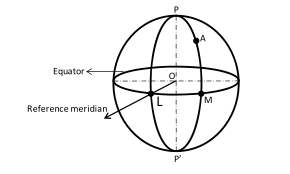
\includegraphics[width=0.8\linewidth]{images/6.png}
    \end{center}
    \begin{center}
        \begin{tabular}{ll}
            \textbf{Arc} & \textbf{Description} \\
            Q. MA & 1. Longitude \\
            R. LM & 2. Co-latitude \\
            S. PA & 3. Latitude \\
        \end{tabular}
    \end{center}
    \begin{enumerate}[label=(\Alph*)]
        \item Q-2, R-3, S-1
        \item Q-3, R-1, S-2
        \item Q-2, R-1, S-3
        \item Q-3, R-2, S-1
    \end{enumerate}

    \item Match the following for the prismatic compass shown below:
    \begin{center}
      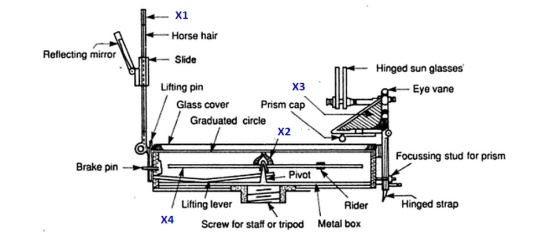
\includegraphics[width=0.8\linewidth]{images/7.png}
    \end{center}
    \begin{center}
        \begin{tabular}{ll}
            \textbf{Component} & \textbf{Name} \\
            P. X1 & 1. Agate bearing \\
            Q. X2 & 2. Object vane \\
            R. X3 & 3. Magnetic needle \\
            S. X4 & 4. Prism \\
        \end{tabular}
    \end{center}
    \begin{enumerate}[label=(\Alph*)]
        \item P-1, Q-2, R-3, S-4
        \item P-1, Q-3, R-2, S-4
        \item P-2, Q-1, R-4, S-3
        \item P-3, Q-1, R-4, S-2
    \end{enumerate}

    \item A ladder placed against a frictionless wall at an inclination of \SI{60}{\degree} with horizontal, is in a state of limiting equilibrium. The ladder has a length of 13 m and a uniform mass of 4 kg/m. The coefficient of friction between the ladder and the floor is \underline{\hspace{1cm}}.

    \item A cubical rock sample is enclosed between two fixed hard steel plates as shown in the figure below. The modulus of elasticity and Poisson’s ratio of the rock are 2 GPa and 0.25, respectively. If the rock is subjected to the stresses as shown in the figure, the strain in x-direction, in mm/m, is \underline{\hspace{1cm}}.
    \begin{center}
      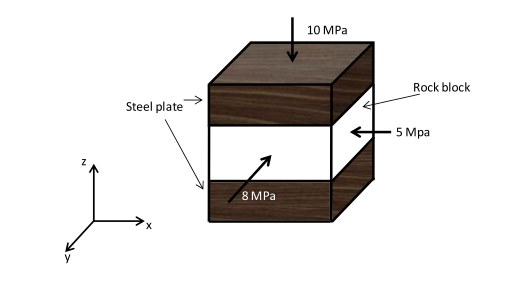
\includegraphics[width=0.8\linewidth]{images/8.png}
    \end{center}

    \item In a hydrostatic stress field, point A is in the middle of two circular openings as shown in the figure. The radial stress, in MPa, at point A is \underline{\hspace{1cm}}.
    \begin{center}
      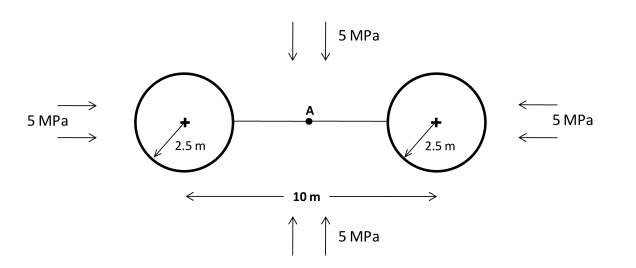
\includegraphics[width=0.8\linewidth]{images/9.png}
    \end{center}

    \item Curves (a) and (b) represent the stress distributions along the length of a ‘full column grouted bolt’ shown in the figure. Curves (a) and (b) are
    \begin{center}
      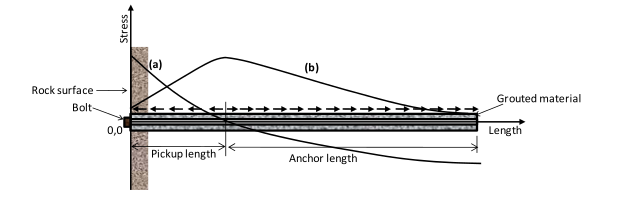
\includegraphics[width=0.8\linewidth]{images/10.png}
    \end{center}
    \begin{enumerate}[label=(\Alph*)]
        \item Tensile stress, Compressive stress
        \item Axial stress, Shear stress
        \item Compressive stress, Tensile stress
        \item Shear stress, Axial stress
    \end{enumerate}

    \item Match the following mechanical properties with the formulae:
    \begin{center}
        \begin{tabular}{ll}
            \textbf{Mechanical property} & \textbf{Formula} \\
            P. Modulus of elasticity & 1. $\sigma_n \tan \phi + c$ \\
            Q. Compressive strength & 2. $\epsilon_{\text{lateral}} / \epsilon_{\text{longitudinal}}$ \\
            R. Shear Strength & 3. $\sigma / \epsilon$ \\
            S. Poisson’s ratio & 4. $F_n / \pi r^2$ \\
        \end{tabular}
    \end{center}
    \begin{enumerate}[label=(\Alph*)]
        \item P-1, Q-2, R-3, S-4
        \item P-1, Q-4, R-3, S-2
        \item P-3, Q-4, R-1, S-2
        \item P-3, Q-2, R-1, S-4
    \end{enumerate}

    \item A skip of 10 tonne capacity hoists ore through a 1000 m deep shaft at a speed of 20 m/s. The skip accelerates and decelerates at \SI{2.0}{\metre\per\second\squared}. The loading and unloading times for the skip are 2.5 min and 1.5 min, respectively. The maximum hourly capacity of the hoisting system, in tonnes, is \underline{\hspace{1cm}}.

    \item Match the following:
    \begin{center}
        \begin{tabular}{ll}
            \textbf{Haulage unit} & \textbf{Safety device} \\
            P. Friction winder & 1. Run-away switch \\
            Q. Drum winder & 2. Lilly controller \\
            R. Direct rope haulage & 3. Regenerative braking \\
            S. Endless rope haulage & 4. Monkey/back catch \\
        \end{tabular}
    \end{center}
    \begin{enumerate}[label=(\Alph*)]
        \item P-1, Q-2, R-3, S-4
        \item P-3, Q-2, R-1, S-4
        \item P-1, Q-3, R-4, S-2
        \item P-2, Q-3, R-1, S-4
    \end{enumerate}

    \item In the gear assembly shown, the rpm of Gear 1 is 600. The number of teeth in Gear 1, Gear 2, Gear 3, Gear 4, Gear 5 and Gear 6 is 30, 45, 15, 20, 10 and 30, respectively. The rpm of Gear 6 is \underline{\hspace{1cm}}.
                \begin{center}
      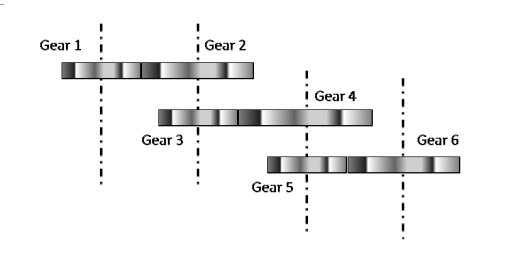
\includegraphics[width=0.8\linewidth]{images/11.png}
    \end{center}

    \item An operating surface mine is proposed to be deepened by 30 m as shown in the figure. If the density of the ore is \SI{2.4}{\tonne\per\metre\cubed}, the incremental stripping ratio for the deepening, in \si{\metre\cubed\per\tonne}, is \underline{\hspace{1cm}}.
                \begin{center}
      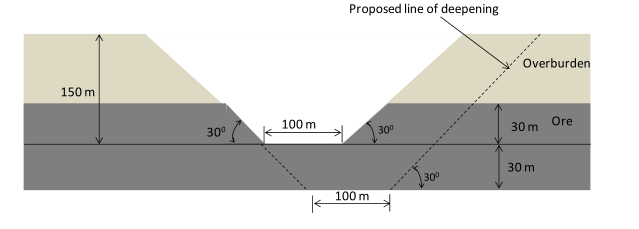
\includegraphics[width=0.8\linewidth]{images/12.png}
    \end{center}

    \item From an openpit sump, mine water is lifted using a 250 m long straight pipeline laid along a gradient of \SI{34}{\degree}. The pumping rate is 500 gpm (1 gallon = 3.8 litres). Additional head loss due to pipe friction can be considered to be 10\% of head lifted. At an overall efficiency of 70\%, the electric power consumed by the pump, in kW, is \underline{\hspace{1cm}}.

    \item With reference to Coward diagram, match the following in the context of explosibility of a mixture of ‘normal air’ and ‘methane’.
    \begin{center}
        \begin{tabular}{ll}
            \textbf{(O$_2$ \%, CH$_4$ \%)} & \textbf{Mixture status} \\
            P. 20.5, 2.4 & 1. Impossible mixture \\
            Q. 19.0, 9.5 & 2. Non-explosive \\
            R. 17.0, 19.0 & 3. Potentially explosive \\
            S. 20.0, 19.5 & 4. Explosive \\
        \end{tabular}
    \end{center}
    \begin{enumerate}[label=(\Alph*)]
        \item P-2, Q-4, R-3, S-1
        \item P-2, Q-3, R-1, S-4
        \item P-2, Q-4, R-1, S-3
        \item P-3, Q-2, R-1, S-4
    \end{enumerate}

    \item A U-tube manometer is subjected to differential pressure as shown. If specific gravity of kerosene is 0.8, the value of $(P_1 - P_2)$, in Pa, is \underline{\hspace{1cm}}.
            \begin{center}
      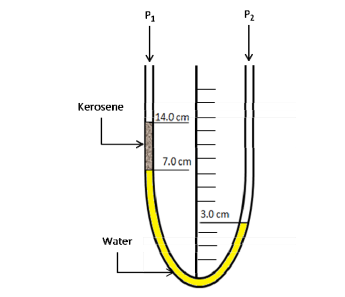
\includegraphics[width=0.8\linewidth]{images/13.png}
    \end{center}

    \item An air stream having an enthalpy of 100 kJ/kgda, is flowing at 20 kgda/s. It is cooled by water at temperature \SI{10}{\celsius} circulating in a cooling coil at a flow rate of 10.0 l/s. If the return temperature of water is \SI{20}{\celsius}, the enthalpy of the cooled air, in kJ/kgda, is \underline{\hspace{1cm}}. (Specific heat of water: 4.18 kJ kg$^{-1}$ \si{\celsius}; kgda: kg of dry air).

    \item The static pressure characteristic of a mine fan is as shown. If the mine resistance is \SI{0.3}{\newton\second\squared\per\metre^8}, the quantity generated by the fan, in \si{\metre\cubed\per\second}, is \underline{\hspace{1cm}}.
        \begin{center}
      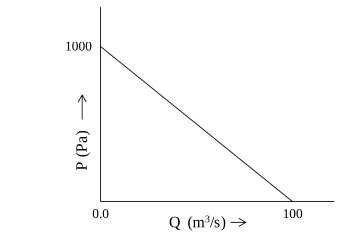
\includegraphics[width=0.8\linewidth]{images/18.png}
    \end{center}

    \item In the context of ventilation plan symbols, match the following:
\begin{flushleft}
  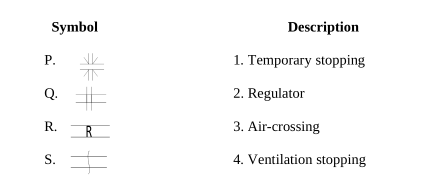
\includegraphics[width=0.8\linewidth]{images/14.png}
\end{flushleft}

    \begin{enumerate}[label=(\Alph*)]
        \item P-3, Q-4, R-2, S-1
        \item P-2, Q-3, R-1, S-4
        \item P-1, Q-3, R-4, S-2
        \item P-3, Q-2, R-1, S-4
    \end{enumerate}

    \item A mill concentrate, having 25\% copper, is proposed to be sold at Rs. 1,25,000 per tonne. The grade of the deposit is 0.8\% Cu and the overall cost of mining and milling is Rs. 2,520 per tonne of ore. At a recovery of 75\%, the estimated profit, in Rs./tonne of concentrate, is \underline{\hspace{1cm}}.

    \item Copper grade distribution in an ore body has the probability density
    function, $f(x)$, as shown in the figure. The average grade of the deposit,
    in \% Cu, is \rule{1.2cm}{0.4pt}. \par
    
    \begin{center}
      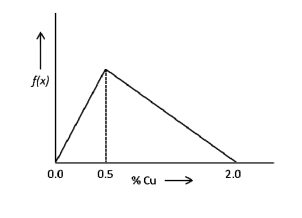
\includegraphics[width=0.8\linewidth]{images/15.png}
    \end{center}

        \item The semivariogram shown belongs to a bauxite deposit.
    The expected difference in the Al$_2$O$_3$ (\%) values between two boreholes
    separated by a distance of 200 m is \rule{1.2cm}{0.4pt}. \par
    
    \begin{center}
      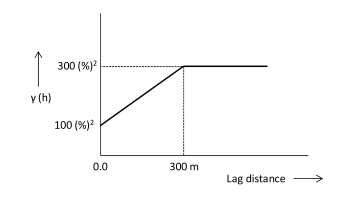
\includegraphics[width=0.8\linewidth]{images/16.png}
    \end{center}
    

    \item A surface mine has 15 identical dumpers and two shovels. For shovel 1, the dumper cycle time is 30 min and the shovel loading time is 5 min. For shovel 2, the dumper cycle time is 32 min and the shovel loading time is 4.0 min. Based on match factor optimisation (equitable match factor), the ideal allocation of dumpers to shovel 1 and shovel 2, respectively is
    \begin{enumerate}[label=(\Alph*)]
        \item 6, 9
        \item 7, 8
        \item 9, 6
        \item 8, 7
    \end{enumerate}
\end{enumerate} 

\makebox[\textwidth]{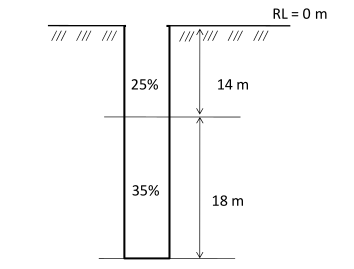
\includegraphics[width=0.8\linewidth]{images/17.png}}

\begin{center}
    \textbf{END OF THE QUESTION PAPER}
\end{center}

\end{document}
